\chapter{Introduction}
\label{chapter_introduction}

\section{Background and Motivation}
\label{sec:intro_background}

Penetration testing -- the authorized, systematic attempt to discover and exploit weaknesses in a target system before a real adversary does -- has traditionally resisted automation because it demands the kind of open-ended, context-sensitive reasoning that scripted scanners cannot perform. Over the past two years, agentic Large Language Models (LLMs) have repeatedly closed parts of this gap. \citet{fang2024hackwebsites} showed that a single LLM agent equipped with a browser and a small set of tools could autonomously perform multi-step SQL-injection attacks against live websites without being told which vulnerability to look for. \citet{fang2024oneday} extended this to real, critical-severity CVEs, showing that GPT-4 could exploit 87\% of a 15-vulnerability benchmark when given the CVE description, though this collapsed to 7\% once the description was withheld -- the first clear evidence that \emph{exploiting} a known vulnerability and \emph{discovering} one are almost entirely different capabilities. \citet{zhu2024hptsa} pushed further into genuinely zero-day territory with a hierarchical team of planning and task-specific agents (HPTSA), and a wide subsequent literature -- surveyed systematically in Chapter~\ref{chapter_backStudy} -- has proposed increasingly elaborate multi-agent, memory-augmented, and planning-augmented architectures for autonomous vulnerability assessment and penetration testing (VAPT).

A systematic reading of this literature -- a corpus of 29 papers spanning single-agent exploitation studies, hierarchical multi-agent frameworks, classical-planning hybrids, cross-mission memory systems, and seven independent benchmark suites -- together with four independently drafted agent-architecture proposals and expert adjudication between them, is the foundation on which this report is built. That reading converges on one finding echoed independently by at least six of the surveyed systems (AWE, AutoPT, VulnBot, PentestAgent, D-CIPHER, and Incalmo): \textbf{architecture, not model scale, is the dominant variable in autonomous exploitation performance.} A well-structured pipeline running a comparatively inexpensive model consistently outperforms an unstructured ReAct-style loop running a frontier model. Yet the same reading surfaces two independent, unresolved failure modes that no single surveyed system addresses simultaneously, and it is the combination of these two gaps -- not either one alone -- that motivates the system proposed in this report.

\section{Problem Statement}
\label{sec:intro_problem}

\textbf{Failure Mode 1 -- Insufficient exploration.} On CVE-Bench \citep{zhu2025cvebench}, a benchmark of 40 critical (CVSS $\geq 9.0$) real-world web-application CVEs, the strongest reported agent exploits only 13\% of one-day and 10\% of zero-day vulnerabilities. CVE-Bench's own failure-mode breakdown identifies \emph{insufficient exploration} as the dominant cause of failure across every agent and evaluation setting, with exploration-failure rates ranging from 37.5\% to 80.0\% (T-Agent: 80.0\% zero-day / 55.0\% one-day; AutoGPT: 72.5\% / 45.0\%; Cy-Agent: 67.5\% / 37.5\%), as illustrated in Figure~\ref{fig:exploration-failure}. Crucially, this is not a reasoning-quality problem -- it is a breadth-of-search problem: agents commit early to a narrow set of candidate attack paths and never return to explore the rest of the surface.

\begin{figure}[htbp]
\centering
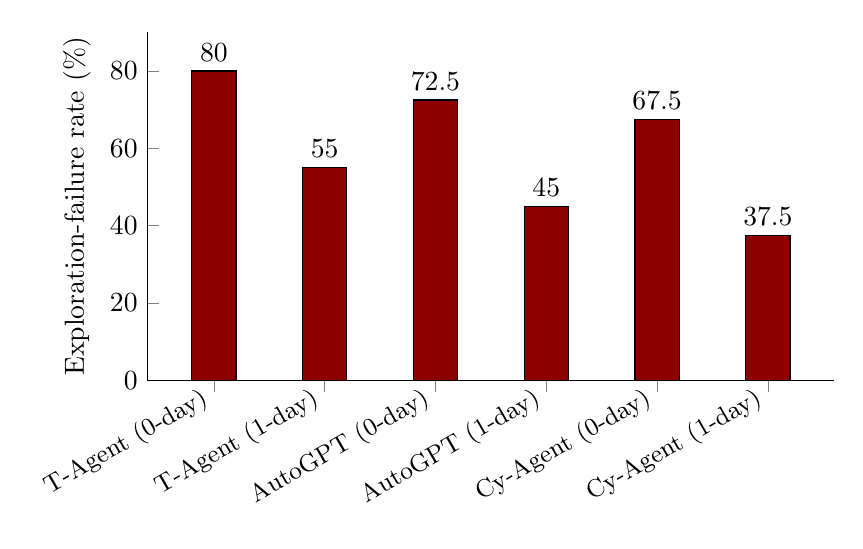
\begin{tikzpicture}
\begin{axis}[
    ybar,
    bar width=16pt,
    width=0.85\textwidth,
    height=6cm,
    ylabel={Exploration-failure rate (\%)},
    symbolic x coords={T-Agent (0-day),T-Agent (1-day),AutoGPT (0-day),AutoGPT (1-day),Cy-Agent (0-day),Cy-Agent (1-day)},
    xtick=data,
    x tick label style={rotate=30,anchor=east,font=\small},
    nodes near coords,
    nodes near coords align={vertical},
    ymin=0, ymax=90,
    axis lines*=left,
    enlarge x limits=0.12,
    ]
\addplot[fill=red!55!black, draw=black] coordinates {
    (T-Agent (0-day),80.0) (T-Agent (1-day),55.0)
    (AutoGPT (0-day),72.5) (AutoGPT (1-day),45.0)
    (Cy-Agent (0-day),67.5) (Cy-Agent (1-day),37.5)
};
\end{axis}
\end{tikzpicture}
\caption{Exploration-failure rate as the dominant CVE-Bench failure mode, by agent and mode (data from CVE-Bench's Table 5 failure-mode breakdown \citep{zhu2025cvebench}).}
\label{fig:exploration-failure}
\end{figure}

\textbf{Failure Mode 2 -- The dependency-reasoning gap.} PentestEval \citep{yang2025pentesteval} decomposes the pentesting pipeline into six stages -- Information Collection (IC), Weakness Gathering (WG), Weakness Filtering (WF), Attack Decision-Making (ADM), Exploit Generation (EG), and Exploit Revision (ER) -- and finds the opposite bottleneck at the \emph{planning} level: ADM, which requires reasoning about prerequisite dependencies between candidate weaknesses, is the single lowest-scoring stage (Spearman correlation 0.25 against expert judgement). PentestEval's ground-truth-injection ablation quantifies exactly how much is available at each stage, summarized in Table~\ref{tab:pentesteval-ablation}.

\begin{table}[htbp]
\centering
\caption{PentestEval ground-truth-injection ablation: marginal gain from replacing each stage's output with expert ground truth, applied cumulatively on top of the SMP baseline \citep{yang2025pentesteval}.}
\label{tab:pentesteval-ablation}
\begin{tabular}{@{}lcc@{}}
\toprule
\textbf{Configuration} & \textbf{End-to-end success} & \textbf{Marginal gain} \\
\midrule
SMP (baseline)                          & 0.31 & --     \\
\quad + GT Weakness Gathering (WG)      & 0.50 & +0.19  \\
\quad + GT Weakness Filtering (WF)      & 0.53 & +0.03  \\
\quad + GT Attack Decision-Making (ADM) & 0.67 & \textbf{+0.14} \\
\bottomrule
\end{tabular}
\end{table}

ADM delivers the largest single-stage marginal increment (+0.14) of the three tested -- measured, notably, on top of an already ground-truthed WG+WF pipeline, not in isolation. Any dynamically-grown dependency structure is necessarily a weaker approximation than ground-truth ADM, so its performance ceiling must be reported honestly as below 0.67 and bounded by the quality of its LLM-inferred edges.

\textbf{The gap no surveyed system closes.} Systems that solve exploration breadth (T-Agent, HPTSA \citep{zhu2024hptsa}, MAPTA \citep{david2025mapta}) dispatch flat, undifferentiated task lists with no explicit prerequisite or dependency model. Systems that solve dependency reasoning (PentestEval's SMP baseline, CHECKMATE-style classical-planning approaches \citep{wang2025checkmate}) are evaluated on curated scenarios with pre-enumerated weakness sets and do not scale to open-ended, wide-surface exploration. No system in the surveyed corpus combines UCB-guided exploration over a dependency-constrained frontier, prerequisite/enables edges grown dynamically from live Specialist discovery, cross-session verified skill accumulation, and evaluation across three independently-benchmarked attack-surface families in one architecture. Closing this compound gap is the problem this report addresses.

\section{Objectives}
\label{sec:intro_objectives}

This report defines, at implementation level, an autonomous VAPT architecture -- \textbf{RedGrid} -- and its accompanying evaluation methodology. The concrete objectives are:

\begin{enumerate}
    \item To design a \textbf{Vulnerability Dependency Graph (VDG)} that unifies dependency-aware exploration with UCB-guided node selection, path-level impact scoring, and failure propagation, formalized to pseudocode level (Chapter~\ref{chapter_proposedMethod}).
    \item To design a \textbf{Dual-Layer World Model} that strictly separates confirmed environmental facts from inferred attack hypotheses, with enforced write-ownership, so that discovery quality and planning quality can be ablated independently.
    \item To design a \textbf{four-layer orchestration architecture} (Orchestrator, Team Manager, Specialists, Execution/Validation) instantiating the structural pattern that every high-performing surveyed system independently converges on.
    \item To design a \textbf{cross-mission memory system} with security-specific conditional branching (e.g., WAF-adaptive payload switching) and oracle-gated skill promotion, distinguishing genuinely reusable strategies from single-target idiosyncrasies.
    \item To define a rigorous, fully pre-existing-benchmark-based \textbf{evaluation plan} -- spanning web, GraphQL, and multi-host attack surfaces -- with statistical methodology (McNemar's test, 95\% Wilson confidence intervals, compute normalization) sufficient for systems-and-empirical-evaluation publication.
    \item To specify the \textbf{ablation studies} required to support each contribution claim, so that no claim in the eventual evaluation is made without a corresponding controlled experiment.
\end{enumerate}

\section{Scope of the Project}
\label{sec:intro_scope}

RedGrid applies one governing rule throughout: it targets \emph{only} attack surfaces for which a dedicated, reusable, oracle-backed benchmark already exists in the surveyed literature. No new benchmark is constructed for this project. Table~\ref{tab:in-scope-surfaces} summarizes the four in-scope attack-surface families and the benchmarks that bound every claim made about them.

\begin{table}[htbp]
\centering
\small
\caption{In-scope attack surfaces and their governing benchmarks.}
\label{tab:in-scope-surfaces}
\begin{tabular}{@{}p{3.1cm}p{5.6cm}p{5.6cm}@{}}
\toprule
\textbf{Attack surface} & \textbf{Benchmark(s)} & \textbf{Representative coverage} \\
\midrule
Web application (HTTP/HTML) & Fang et al.\ 15-vuln sandbox \citep{fang2024oneday}; HPTSA 14-CVE zero-day suite \citep{zhu2024hptsa}; CVE-Bench (40 CVEs) \citep{zhu2025cvebench}; MAPTA/XBOW (104) \citep{david2025mapta}; HackWorld (36) \citep{ren2025hackworld}; PentestEval (346 tasks) \citep{yang2025pentesteval}; Cybench \citep{zhang2025cybench}; PentestGPT/HTB machine sets \citep{deng2024pentestgpt} & SQLi, XSS, CSRF, SSRF, SSTI, LFI, file-upload RCE, IDOR, auth bypass, framework RCEs, JWT forgery \\
GraphQL APIs & PrediQL 6-API suite \citep{liu2025prediql} & Schema abuse, dependency-chain injection, batched-auth bypass, IDOR, nested-query DoS \\
Multi-host / Active Directory & Incalmo MHBench (40 environments) \citep{singer2025incalmo} & Lateral movement, credential reuse, privilege escalation \\
Production system corpus (hard tier) & BountyBench (25 real systems) \citep{zhang2025bountybench} & Economic/adversarial validation layer over the web surface \\
\bottomrule
\end{tabular}
\end{table}

\textbf{Explicitly out of scope.} General REST API exploitation is not evaluated and no REST-specific pass rate is ever reported: RESTler's \citep{atlidakis2019restler} evaluation targets are one-off real-world case studies rather than a standardized, reusable benchmark, so there is no "RESTBench" equivalent in the surveyed corpus. RESTler's dependency-inference and response-feedback-pruning techniques are nonetheless methodologically valuable and are reused \emph{internally} by the GraphQL Specialist and by the Team Manager's edge-inference logic (Section~\ref{sec:vdg-algorithm}). Binary exploitation, physical- and network-layer attacks, and social engineering are likewise out of scope for the same reason: no dedicated, oracle-backed benchmark for them exists in the surveyed literature.

\section{Expected Contributions}
\label{sec:intro_contributions}
\label{sec:not-a-contribution}

Consistent with the design principle that a paper claiming many contributions invites the conclusion that it is a "bundle of incremental integrations," this report makes exactly three primary scientific contributions, each bounded by a precisely specified experimental test (formalized in Chapter~\ref{chapter_experimentalResults}):

\begin{itemize}
    \item \textbf{C1 -- Dependency-Aware Attack Graph Exploration (Primary).} A dynamically constructed VDG combining UCB-guided selection over a dependency-constrained frontier, path-level impact scoring, and ordinal evidence backpropagation, targeting zero-day pass@1 $\geq 25\%$ on CVE-Bench and an ADM score $\geq 0.50$ on PentestEval, contingent on a mandatory pre-evaluation edge-inference precision gate.
    \item \textbf{C2 -- Cross-Mission Memory with Verified Skill Promotion (Supporting).} A three-tier memory architecture with security-specific conditional-branching strategies and oracle-gated skill promotion, targeting measurable improvement on seen-technology targets relative to a no-memory baseline.
    \item \textbf{C3 -- Comprehensive Cross-Benchmark Evaluation with Standardized Oracles (Methodological).} The first evaluation of a single autonomous VAPT architecture across web, GraphQL, and multi-host surfaces under one shared orchestration layer, with surface-specific Specialist pools and strictly separated per-surface reporting.
\end{itemize}

Several further mechanisms -- declarative task dispatch, the Structured Handoff Bridge, the Diagnosis-Adapt-Cap validation loop, the Usage Tracker, and the Engagement Trajectory Log -- are retained as supporting infrastructure that the evaluation depends on, but are deliberately \emph{not} claimed as primary novelty contributions; the rationale for each demotion is given in Section~\ref{sec:not-a-contribution}.

\section{Challenges}
\label{sec:intro_challenges}
\label{sec:threats-validity}

Nine threats to validity are tracked explicitly throughout this report and are treated as first-class design constraints rather than post-hoc caveats (full detail in Section~\ref{sec:threats-validity}):

\begin{enumerate}
    \item \textbf{VDG edge-inference accuracy} is LLM-inferred rather than ground-truth-annotated, and is the single highest-risk item in the entire architecture; a mandatory pilot study against PentestEval's ground-truth dependency annotations must show $\geq 50\%$ precision before the main evaluation may proceed.
    \item \textbf{Sandbox-to-real-world gap.} \citet{fang2024hackwebsites} found 1 exploitable XSS in 50 real-world candidate sites (2\%) versus 73.3\% in a matched sandbox; RedGrid must report both regimes and must not extrapolate from one to the other.
    \item \textbf{GraphQL evaluation is statistically narrow} -- PrediQL's 6-API suite is real and standardized but far smaller than CVE-Bench or XBOW, so generalization claims involving GraphQL must state this asymmetry plainly.
    \item \textbf{Cost-per-exploit is backbone-price-sensitive} and must be reported with an explicit model, version, and date rather than as an absolute claim.
    \item \textbf{Negative transfer in cross-mission memory} -- a strategy validated against one framework version may be actively harmful against another; this risk is unaddressed in all 29 surveyed papers because none implement cross-mission, strategy-level memory generalization for VAPT.
    \item \textbf{UCB hyperparameter sensitivity} across seven tunable parameters, requiring an explicit search-range report and a $\pm 10\%$ perturbation sensitivity analysis.
    \item \textbf{Statistical power on small benchmarks} -- PrediQL's 6 APIs at 5 runs yield only 30 data points, likely underpowering McNemar's test for small effect sizes.
    \item \textbf{Edge-inference scalability} -- unbatched pairwise edge inference would require $O(2M)$ frontier-model calls per new node, plausibly exceeding the entire per-CVE compute budget; batching is required and its own quality trade-offs must be measured.
    \item \textbf{Honest framing of "one architecture, three surfaces"} -- different Specialist pools activate per attack surface, so C3 is reported as a shared orchestrator with surface-specific modules, not as one literally unmodified architecture.
\end{enumerate}

\section{Organization}
\label{sec:intro_organization}

The remainder of this report is organized as follows. Chapter~\ref{chapter_backStudy} surveys the 29-paper corpus underlying this work, organizing it by architectural pattern, and derives the fifteen-item prior-work gap table that motivates RedGrid's design. Chapter~\ref{chapter_proposedMethod} presents the complete RedGrid architecture: the four-layer orchestration hierarchy, the Dual-Layer World Model, the formalized VDG algorithm (node schema, UCB formula, edge-construction and update rules, path scoring, and failure propagation), the per-Specialist methodology for each of the four in-scope attack surfaces, and the memory and state services. Chapter~\ref{chapter_implementations} lays out the execution plan for building and validating this architecture -- work breakdown, timeline, milestones, resourcing, and risk assessment. Chapter~\ref{chapter_experimentalResults} specifies the evaluation plan: the seven-tier benchmark suite, the statistical methodology, and the eight required ablation studies. Chapter~\ref{chapter_conclusion} summarizes the report, lists the expected deliverables, and outlines directions for future work beyond the scope defined here.
